%%%%%%%%%%%%%%%%%%%%%%%%%%%%%%%%%%%%%%%%%
% Maggi Memoir Thesis (WriteLaTeX Version - Compiles with pdflatex)
% XeLaTeX Template
% Version 1.0 (22/12/13)
%
% This template has been downloaded from:
% http://www.LaTeXTemplates.com
%
% Original authors:
% Federico Maggi (fede@maggi.cc) with extensive modifications by:
% Vel (vel@latextemplates.com)
%
% License:
% CC BY-NC-SA 3.0 (http://creativecommons.org/licenses/by-nc-sa/3.0/)
%
% Important note:
% Most of the document content and packages are specified within structure.tex
% so if you need to make modifications to the template have a look there first!
%
%%%%%%%%%%%%%%%%%%%%%%%%%%%%%%%%%%%%%%%%%

%----------------------------------------------------------------------------------------
%	PACKAGES AND OTHER DOCUMENT CONFIGURATIONS
%----------------------------------------------------------------------------------------

\documentclass[10pt,a4paper,twoside]{memoir} % Change font size here (allowable values are 9pt-12pt), change the paper size, specify one or two sided printing and specify whether to show trimming lines

%----------------------------------------------------------------------------------------
%	VARIOUS REQUIRED PACKAGES AND CONFIGURATIONS
%----------------------------------------------------------------------------------------

\usepackage[utf8]{inputenc}
\usepackage[italian]{babel}
\usepackage[T1]{fontenc}
\usepackage[round]{natbib}\citeindextrue % Round brackets around citations, change to square for square brackets
\usepackage{graphicx} % Required to include images
%\usepackage{color} % Required for custom colors
\usepackage[dvipsnames]{xcolor}
\definecolor{aawhite}{rgb}{0.97,0.97,0.97}
\definecolor{awhite}{rgb}{0.90,0.90,0.90}
\definecolor{lgreen}{rgb}{0.94,1.0,0.98}
\definecolor{dgreen}{rgb}{0.0,0.3,0.1}
\definecolor{sgreen}{rgb}{0.0,0.7,0.3}
\definecolor{lgreen}{rgb}{0.94,1.0,0.98}
\definecolor{bgreen}{rgb}{0.00,0.50,0.25}
\definecolor{dblue}{rgb}{0.0,0.1,0.6}
\definecolor{lblue}{rgb}{0.8,0.8,1.0}
\definecolor{mixed}{rgb}{0.0,0.3,0.3}
\definecolor{dred}{rgb}{0.6,0.2,0.0}
\definecolor{sred}{rgb}{0.7,0.2,0.0}
\definecolor{ddred}{rgb}{0.3,0.1,0.0}
\definecolor{turq}{rgb}{0.28,0.82,0.80}
\definecolor{lyellow}{rgb}{1.00,0.97,0.94}
\definecolor{mygreen}{rgb}{0,0.6,0}
\definecolor{mygray}{rgb}{0.5,0.5,0.5}
\definecolor{mymauve}{rgb}{0.58,0,0.82}
\definecolor{codegreen}{rgb}{0,0.6,0}
\definecolor{codegray}{rgb}{0.5,0.5,0.5}
\definecolor{codepurple}{rgb}{0.58,0,0.82}
\definecolor{backcolour}{rgb}{0.96,0.96,0.96}

\usepackage{amsmath,amssymb,theorem} % Math packages
\usepackage{listings} % Required for including snippets of code
\usepackage{booktabs} % Required for better horizontal rules in tables
\usepackage{xspace} % Provides the ability to use an intelligent space which is used in \institution and \department
\usepackage[printonlyused,withpage]{acronym} % Include a list of acronyms
\usepackage{rotating} % Allows tables and figures to be rotated
\usepackage{hyperref} % Required for links and changing link options
\hypersetup{
    colorlinks=true,
    linkcolor=sred,
    filecolor=magenta,
    urlcolor=cyan,
    citecolor=sgreen,
    bookmarks=true,
}
%\hypersetup{colorlinks, breaklinks, linkcolor=black,citecolor=black,filecolor=black,urlcolor=black} % Set up hyperlinks including colors for references, urls and citations

\usepackage{microtype} % Slightly tweak font spacing for aesthetics

\usepackage{listings}
\lstdefinelanguage{Coq}{
    morekeywords = [1]{Inductive, Fixpoint, Theorem, Lemma, Example},
    morekeywords = [2]{match, with, end},
    morekeywords = [3]{Require, Import, Set, Implicit, Arguments, Qed, Proof},
    morekeywords = [4]{},
    morekeywords = [5]{ },
    keywordstyle = [1]\color{dred},
    keywordstyle = [2]\color{dgreen},
    keywordstyle = [3]\color{codepurple},
    keywordstyle = [4]\color{orange},
    keywordstyle = [5]\color{lblue},
    sensitive = true,
    morecomment = [l]{//},
    morecomment = [s]{(*}{*)},
    morecomment = [s]{(**}{*)},
    commentstyle={\color{dgreen}},
    morestring = [b]",
    morestring = [b]',
    basicstyle={\small\ttfamily\bfseries},
    stringstyle={\ttfamily\small\color{orange}},
    numbers=left,
    numberstyle=\tiny\color{mygray},
    xrightmargin=0em,
    xleftmargin=3em,
    stepnumber=1,
    numbersep=1em,
    lineskip=-0.5ex,
    mathescape=true,
    showstringspaces=false,
    %    frame={tb},
    frame=none,
    breaklines=true,
    columns=[l]{fullflexible},
    keepspaces=true,
    literate=
        {á}{{\'a}}1
        {à}{{\`a}}1
        {é}{{\'e}}1
        {è}{{\`e}}1
        {ì}{{\`i}}1
        {ò}{{\`o}}1
        {ù}{{\`u}}1
        {∀}{{forall}}1
}

\lstnewenvironment{Coq}{\lstset{language={Coq},}}{}

\lstdefinestyle{Coq-style}{
	backgroundcolor=\color{backcolour},
	commentstyle=\color{codegreen},
	keywordstyle=\color{magenta},
	numberstyle=\tiny\color{codegray},
	stringstyle=\color{codepurple},
	basicstyle=\fontsize{9}{13}\selectfont\ttfamily,
%	basicstyle=\ttfamily\footnotesize,
	breakatwhitespace=false,
	breaklines=true,
	captionpos=b,
	keepspaces=true,
	numbers=left,
	numbersep=5pt,
	showspaces=false,
	showstringspaces=false,
	showtabs=false,
	tabsize=2
}
\renewcommand{\verb}{\lstinline}
\newcommand{\verbCoq}[1]{\lstinline[language=Coq,style=Coq-style]+#1+}
\newcommand{\vCoq}[1]{\lstinline[language=Coq,style=Coq-style]+#1+}
%%% lstlisting stop definitions


\makeatletter
\renewcommand{\fnum@figure}{\textsc{\figurename~\thefigure}} % Make the "Figure 1.1" text in small caps
\makeatother

%----------------------------------------------------------------------------------------
%	PAGE LAYOUT
%----------------------------------------------------------------------------------------

% The memoir class used in this template contains the ability to set the stock paper size and the trimmed size independently. It also has the ability to show trim lines showing where stock paper should be trimmed to get the final book size. This can all be a bit confusing so please see the memoir class documentation for more information.

% By default, the paper size is a4paper which is 29.7cm × 21cm. To change this, simply change "a4paper" in the \documentclass[a4paper,...]{memoir} command in thesis.tex to another size such as "letterpaper".
% By default, the trimmed size is 24cm x 17cm and trim lines are shown. To remove trim lines, simply remove "showtrims" from the \documentclass[showtrims,...]{memoir} command in thesis.tex. The size of the trimmed content is set with the \settrimmedsize{}{} command below.
% If you wish to remove trims and set the content to fit the paper size (i.e. no trimming at all), all you have to do is remove "showtrims" as above and comment out the \settrimmedsize{}{} command below.

%\setstocksize{24cm}{17cm} % Uncomment to manually set the stock size and override the setting in \documentclass
\settrimmedsize{24cm}{17cm}{*} % Change the trimmed area size or comment out this line entirely to fit the content to the paper size without trimming
\setlrmarginsandblock{37.125mm}{*}{0.9} % The first bracket specifies the spine margin, the second the edge margin and the third the ratio of the spine to the edge. Only one or two values are required and the remaining one(s) can be a star (*) to specify it is not needed. By default the edge margin is 10% smaller and
\setulmarginsandblock{37.125mm}{*}{*} % The first bracket specifies the upper margin, the second the lower margin and the third the ratio of the upper to the lower. Only one or two values are required and the remaining one(s) can be a star (*) to specify it is not needed.
\setmarginnotes{17pt}{51pt}{\onelineskip} % The size of marginal notes, the three values in curly brackets are \marginparsep, \marginparwidth and \marginparpush
\setheadfoot{\onelineskip}{2\onelineskip} % Sets the space available for the header and footer
\setheaderspaces{*}{2\onelineskip}{*} % Sets the spacing above and below the header
\setlength{\trimtop}{0pt} % Sets the spacing above the trimmed area, i.e. moved the trimmed area down the page if positive

% Comment the two lines below to reverse the position of the trimmed content on the stock paper, i.e. odd pages will have content on the right side instead of the left and even pages will have content on the left side instead of the right
\setlength{\trimedge}{\stockwidth}
\addtolength{\trimedge}{-\paperwidth}

\checkandfixthelayout % Makes sure your specifications are correct and implements them in the document

%----------------------------------------------------------------------------------------
%	CHAPTER HEADING STYLE
%----------------------------------------------------------------------------------------

\makeatletter
\makechapterstyle{thesis}{
\renewcommand{\chapternamenum}{}
\setlength{\beforechapskip}{0pt}
\setlength{\midchapskip}{0pt}
\setlength{\afterchapskip}{0pt}
\renewcommand{\chapnamefont}{\LARGE}
\renewcommand{\chapnumfont}{\chapnamefont}
\renewcommand{\chaptitlefont}{\chapnamefont}
\renewcommand{\printchapternum}{}
\renewcommand{\afterchapternum}{}
\renewcommand{\printchaptername}{}
\renewcommand{\afterchaptertitle}{\chapnumfont\hfill\thechapter\\\vspace*{-.3cm}\hrulefill\vspace*{6cm}\\}
}
\makeatother

%----------------------------------------------------------------------------------------
%	TABLE OF CONTENTS DEPTH
%----------------------------------------------------------------------------------------

\maxsecnumdepth{subsubsection}
\maxtocdepth{subsection}

%----------------------------------------------------------------------------------------
%	MATH THEOREM DEFINITIONS
%----------------------------------------------------------------------------------------

\theoremstyle{plain}
\newtheorem{thm}{Theorem}[section] % Defines the theorem environment
\newtheorem{prop}[thm]{Proposition} % Defines the proposition environment
\newtheorem{proof}{Proof}[section] % Defines the proof environment
\newtheorem{definition}{Definition}[section] % Defines the definition environment
\newtheorem{example}{Example}[section] % Defines the example environment
\newtheorem{rem}{Remark} % Defines the remark environment
\newtheorem{note}{Note}[section] % Defines the note environment

%----------------------------------------------------------------------------------------
%	CODE SNIPPET CONFIGURATION
%----------------------------------------------------------------------------------------

\lstset{
  basicstyle=\ttfamily\small,
  basewidth=0.55em,
  showstringspaces=false,
  numbers=left,
  numberstyle=\tiny,
  numbersep=2.5pt,
  keywordstyle=\bfseries\ttfamily,
  breaklines=true
}
% Examples of list environments for different programming languages, you will likely need to specify your own
\lstnewenvironment{pseudoc}{\lstset{frame=lines,language=C,mathescape=true}}{}
\lstnewenvironment{logs}{\lstset{frame=lines,basicstyle=\footnotesize\ttfamily,numbers=none}}{}
\lstnewenvironment{cc}{\lstset{frame=lines,language=C}}{}
\lstnewenvironment{c64}{\lstset{backgroundcolor=\color{c64},basewidth=0.65em,basicstyle=\commodoreface\color{c64light},numbers=none,framerule=10pt,rulecolor=\color{c64light},frame=tb,framexbottommargin=30pt}}{}
\lstnewenvironment{html}{\lstset{frame=lines,language=html,numbers=none}}{}
\lstnewenvironment{pseudo}{\lstset{frame=lines,mathescape=true,morekeywords={learn_string_domain, save_model}}}{}
\lstnewenvironment{pseudoctiny}{\lstset{language=C,mathescape=true,basicstyle=\tiny\sffamily}}{}
\lstnewenvironment{cctiny}{\lstset{language=C,basicstyle=\tiny\sffamily}}{}
\lstnewenvironment{pseudotiny}{\lstset{mathescape=true,basicstyle=\tiny\sffamily}}{} % Include the file containing the code defining the structure and style of the document

%------------------------------------------------
% Thesis Information

\title{TITOLO} % Thesis title

\author{Nome Cognome} % Author name

\date{Maggio 2021} % The date

\newcommand{\institution}{Politecnico di torino\xspace} % University/institution name

\newcommand{\department}{Dipartimento di \ldots (\textsf{DIMEA})\xspace} % Department name

%------------------------------------------------
% Fonts

\renewcommand*{\acffont}[1]{{\normalsize\itshape #1}} % Font style for the acronym text (e.g. Do It Yourself)
\renewcommand*{\acfsfont}[1]{{\normalsize\upshape #1}} % Font style for the acronym in bracket (e.g. (DIY))

%------------------------------------------------
% Hyphenations

\hyphenation{a-no-ma-lous a-no-ma-ly amounts breaches} % Specify custom hyphenation points in words with dashes where you would like hyphenation to occur, or alternatively, don't put any dashes in a word to stop hyphenation altogether

%----------------------------------------------------------------------------------------
%	TITLE PAGE
%----------------------------------------------------------------------------------------

\renewcommand{\maketitlehooka}{
\centering
%%%%%% QUI C'È IL LOGO

\includegraphics[width=2.5cm]{Figures/polimi-logo}\\[.5cm] % Institution logo
\institution\\ % Print institution name
\emph{\department}\\[.2cm] % Print department name
CORSO DI LAUREA IN INGEGNERIA AEROSPAZIALE
%DOTTORATO DI RICERCA IN INGEGNERIA DELL'INFORMAZIONE % Degree or other information
\par
\hrulefill
\vfill}
\renewcommand{\maketitlehookb}{\vfill}
\renewcommand{\maketitlehookc}{
\vfill
\begin{flushleft}
Advisor:\\
\textbf{Prof. ????}\\[.3cm] % Advisor's/supervisor's name
Tutor:\\
\textbf{Prof. ????}\\[.3cm] % Tutor's name
Supervisor of the Doctoral Program:\\
\textbf{Prof. ???} % Doctoral program supervisor's name
\end{flushleft}
\vfill}
\preauthor{\begin{flushright}Relazione tecnica:\\\bfseries} % Text prior \preauthor{\begin{flushright}Doctoral Dissertation of:\\\bfseries} % Text prior to the author name - right aligned and bold
\postauthor{\end{flushright}} % After the author name, stop right alignment

%----------------------------------------------------------------------------------------

\makeindex % Write an index file

\begin{document}

\begin{titlingpage}
\maketitle % Print the title page
\end{titlingpage}

\frontmatter % Use roman page numbering style (i, ii, iii, iv...) for the pre-content pages

%----------------------------------------------------------------------------------------
%	PREFACE
%----------------------------------------------------------------------------------------
%
\section*{Preface}
This thesis embraces all the efforts that I put during the last three years as a PhD student at Politecnico di Milano. I have been working under the supervision of Prof. S. Zanero and Prof. G. Serazzi, who is also the leader of the research group I am part of. In this time frame I had the wonderful opportunity of being ``initiated'' to research, which radically changed the way I look at things: I found my natural \emph{``thinking outside the box''} attitude --- that was probably well-hidden under a thick layer of lack-of-opportunities, I took part of very interesting joint works --- among which the year I spent at the Computer Security Laboratory at UC Santa Barbara is at the first place, and I discovered the Zen of my life.

My research is all about \emph{computers} and every other technology possibly related to them. Clearly, the way I look at computers has changed a bit since when I was seven. Still, I can remember me, typing on that \textsf{Commodore} 64 in front of a tube TV screen, trying to get that d---n routine written in \textsf{Basic} to work. I was just playing, obviously, but when I recently found a picture of me in front of that screen...it all became clear.

So, although my attempt of writing a program to authenticate myself was a little bit naive --- being limited to a print instruction up to that point apart, of course --- I thought \emph{``maybe I am not in the wrong place, and the fact that my research is still about security is a good sign''}!

Many years later, this work comes to life. There is a humongous amount of people that, directly or indirectly, have contributed to my research and, in particular, to this work. Since my first step into the lab, I will not, ever, be thankful enough to Stefano, who, despite my skepticism, convinced me to submit that application for the PhD program. For trusting me since the very first moment I am thankful to Prof. G. Serazzi as well, who has been always supportive. For hosting and supporting my research abroad I thank Prof. G. Vigna, Prof. C. Kruegel, and Prof. R. Kemmerer. Also, I wish to thank Prof. M. Matteucci for the great collaboration, Prof. I. Epifani for her insightful suggestions and Prof. H. Bos for the detailed review and the constructive comments.

On the colleagues-side of this acknowledgments I put all the fellows of Room 157, Guido, the crew of the seclab and, in particular, Wil with whom I shared all the pain of paper writing between Sept '08 and Jun '09.

On the friends-side of this list Lorenzo and Simona go first, for being our family.

I have tried to translate in simple words the infinite gratitude I have and will always have to Valentina and my parents for being my fixed point in my life. Obviously, I failed.

\begin{flushright}
\textsc{\theauthor}\\
Milano\\
September 2009
\end{flushright}

\cleartoverso % Force a break to an even page


%----------------------------------------------------------------------------------------
%	ABSTRACT
%----------------------------------------------------------------------------------------
\begin{abstract}
%This dissertation details our research on anomaly detection techniques, that are central to several classic security-related tasks such as network monitoring, but it also have broader applications such as program behavior characterization or malware\index{malware} classification. In particular, we worked on anomaly detection from three different perspective, with the common goal of recognizing awkward activity on computer infrastructures. In fact, a computer system has several weak spots that must be protected to avoid attackers to take advantage of them. We focused on protecting the operating system, central to any computer, to avoid malicious code to subvert its normal activity. Secondly, we concentrated on protecting the web applications, which can be considered the modern, shared operating systems; because of their immense popularity, they have indeed become the most targeted entry point to violate a system. Last, we experimented with novel techniques with the aim of identifying related events (e.g., alerts reported by intrusion detection systems) to build new and more compact knowledge to detect malicious activity on large-scale systems.
%
%Our contributions regarding host-based protection systems focus on characterizing a process' behavior through the system calls invoked into the kernel. In particular, we engineered and carefully tested different versions of a multi-model detection system using both stochastic and deterministic models to capture the features of the system calls during normal operation of the operating system. Besides demonstrating the effectiveness of our approaches, we confirmed that the use of finite-state, deterministic models allow to detect deviations from the process' control flow with the highest accuracy; however, our contribution combine this effectiveness with advanced models for the system calls' arguments resulting in a significantly decreased number of false alarms.
%
%Our contributions regarding web-based protection systems focus on advanced training procedures to enable learning systems to perform well even in presence of changes in the web application source code --- particularly frequent in the Web 2.0 era. We also addressed data scarcity issues that is a real problem when deploying an anomaly detector to protect a new, never-used-before application. Both these issues dramatically decrease the detection capabilities of an intrusion detection system but can be effectively mitigated by adopting the techniques we propose.
%
%Last, we investigated the use of different stochastic and fuzzy models to perform automatic alert correlation, which is as post processing step to intrusion detection. We proposed a fuzzy model that formally defines the errors that inevitably occur if time-based alert aggregation (i.e., two alerts are considered correlated if they are close in time) is used. This model allow to account for measurements errors and avoid false correlations due to delays, for instance, or incorrect parameter settings. In addition, we defined a model to describe the alert generation as a stochastic process and experimented with non-parametric statistical tests to define robust, zero-configuration correlation systems.
%
%The aforementioned tools have been tested over different datasets --- that are thoroughly documented in this document --- and lead to interesting results.


Qua metti quello che hai fatto.
\end{abstract}

\cleartoverso % Force a break to an even page


%----------------------------------------------------------------------------------------
%	TABLE OF CONTENTS
%----------------------------------------------------------------------------------------

\tableofcontents* % Print the table of contents
\cleartoverso % Force a break to an even page

%----------------------------------------------------------------------------------------
%	LIST OF FIGURES
%----------------------------------------------------------------------------------------
%\listoffigures % Print the list of figures
\cleartoverso % Force a break to an even page

%----------------------------------------------------------------------------------------
%	LIST OF TABLES
%----------------------------------------------------------------------------------------

%\listoftables % Print the list of tables
\cleartoverso % Force a break to an even page


%----------------------------------------------------------------------------------------
%	ACRONYMS
%----------------------------------------------------------------------------------------

%\chapter{List of Acronyms}
\begin{acronym}\addtolength{\itemsep}{-\baselineskip}
  \acro{AIC}{Akaike Information Criterion}
  \acro{ARMA}{Auto Regressive Moving Average}
  \acro{ARMAX}{Auto Regressive Moving Average eXogenous}
  \acro{ARX}{Auto Regressive eXogenous}
  \acro{AR}{Auto Regressive}
  \acro{ARR}{Alert Reduction Rate}
  \acro{ANSI}{American National Standard Institute}
  \acro{ASCII}{American Standard for Information Interxchange}
  \acro{BIC}{Bayesian Information Criterion}
  \acro{BMU}{Best Matching Unit}
  \acro{BSM}{Basic Security Module}
  \acro{CDF}{Cumulative Density Function}
  \acro{CDX}{Cyber Defense eXercise}
  \acro{CIA}{Confidentially Integrity Availability}
  \acro{CIDS}{Collaborative IDS}
  \acro{CPU}{Central Processing Unit}
  \acro{CSV}{Comma Separated Values}
  \acro{CTF}{Capture The Flag}
  \acro{DAG}{Direct Acyclic Graph}
  \acro{DARPA}{Defense Advanced Research Projects Agency}
  \acro{DB}{DataBase}
  \acro{DBMS}{DataBase Management System}
  \acro{DIDS}{Distributed IDS}
  \acro{DNS}{Domain Name System}
  \acro{DOM}{Document Object Model}
  \acro{DoS}{Denial of Service}
  \acro{DR}{Detection Rate}
  \acro{DTD}{Document Type Definition}
  \acro{ED}{Elementary Detector}
  \acro{ELF}{Executable Linux Format}
  \acro{FN}{False Negative}
  \acro{FNR}{False Negative Rate}
  \acro{FPR}{False Positive Rate}
  \acro{FP}{False Positive}
  \acro{FSA}{Finite State Automaton}
  \acro{FTP}{File Transfer Protocol}
  \acro{GCI}{Granger Causality Index}
  \acro{GCT}{Granger Causality Test}
  \acro{HIDS}{Host-based Intrusion Detection System}
  \acro{HMM}{Hidden Markov Model}
  \acro{HTML}{HyperText Markup Language}
  \acro{HTTP}{HyperText Transfer Protocol}
  \acro{ICD}{Idealized Character Distribution}
  \acro{IDEVAL}{Intrusion Detection eVALuation}
  \acro{IDMEF}{Intrusion Detection Message Exchange Format}
  \acro{IDS}{Intrusion Detection System}
  \acro{IDWG}{Intrusion Detection Working Group}
  \acro{ID}{Intrusion Detection}
  \acro{IETF}{Internet Engineering Task Force}
  \acro{IODEF}{Incident Object Description and Interchange Format}
  \acro{IPS}{Intrusion Protection System}
  \acro{ISP}{Internet Service Provider}
  \acro{IP}{Internet Protocol}
  \acro{IR}{Information Retrieval}
  \acro{IRC}{Internet Relay Chat}
  \acro{ISS}{Internet Security Systems}
  \acro{JSON}{JavaScript Object Notation}
  \acro{KBS}{Knowledge Base System}
  \acro{KS}{Kolmogorov-Smirnoff}
  \acro{LARIAT}{Lincoln Adaptable Real-time Information Assurance Testbed}
  \acro{LERAD}{Learning Rules for Anomaly Detection}
  \acro{LL}{Lincoln Laboratory}
  \acro{MDL}{Minimum Description Length}
  \acro{MIT}{Massachusetts Institute of Technology}
  \acro{ML}{Maximum Likelihood}
  \acro{MTU}{Maximum Transfer Unit}
  \acro{NIDES}{Next-generation Intrusion Detection Expert System}
  \acro{NIDS}{Network-based Intrusion Detection System}
  \acro{NNID}{Neural Network Intrusion Detection}
  \acro{NSTISSC}{National Security Telecomm. and Information Systems Sec. Committee}
  \acro{NTP}{Network Time Protocol}
  \acro{PC}{Program Counter}
  \acro{PDF}{Probability Density Function}
  \acro{PHAD}{Packet Header Anomaly Detection}
  \acro{PHP}{PHP Hypertext Preprocessor}
  \acro{PID}{Process IDentifier}
  \acro{ROC}{Receiving Operating Characteristic}
  \acro{SADE}{Syscall Sequence Arguments Anomaly Detection Engine}
  \acro{SDEE}{Security Device Event Exchange}
  \acro{SMTP}{Simple Message Transfer Protocol}
  \acro{SOM}{Self Organizing Map}
  \acro{SQL}{Structured Query Language}
  \acro{SRI}{Stanford Research Institute}
  \acro{SSH}{Secure SHell}
  \acro{STATL}{State Transition Analysis Technique Language}
  \acro{SVN}{SubVersioN}
  \acro{SYN}{SYNchronize}
  \acro{TCP}{Trasmission Control Protocol}
  \acro{TF}{Truth File}
  \acro{TN}{True Negative}
  \acro{TNR}{True Negative Rate}
  \acro{TOS}{Type Of Service}
  \acro{TP}{True Positive}
  \acro{TTL}{Time To Live}
  \acro{UCSB}{University of California Santa Barbara}
  \acro{ULISSE}{Unsupervised Learning IDS with 2-Stages Engine}
  \acro{UDP}{User Datagram Protocol}
  \acro{UML}{Unified Modeling Language}
  \acro{URL}{Uniform Resource Locator}
  \acro{VPN}{Virtual Private Network}
  \acro{XML}{eXtensible Markup Language}
  \acro{XSD}{XML Schema Definition}
  \acro{XSS}{Cross-Site Scripting}
\end{acronym}
\cleartoverso % Force a break to an even page % Include a List of Acronyms section using acronyms.tex where they are defined

%----------------------------------------------------------------------------------------
%	COLOPHON
%----------------------------------------------------------------------------------------

%\thispagestyle{empty} % Remove all headers and footers from this page

\vspace*{2em}
\renewcommand{\abstractname}{Colophon}
\begin{abstract}
This document was typeset using the \textsf{XeTeX} typesetting system created by the Non-Roman Script Initiative and the memoir class created by Peter Wilson. The body text is set 10pt with~Adobe Caslon Pro. Other fonts include \texttt{Envy Code R}, \textsf{Optima Regular} and. Most of the drawings are typeset using the \textsf{TikZ/PGF} packages by Till Tantau.
\end{abstract}
\vfill


%----------------------------------------------------------------------------------------
%	CONTENT CHAPTERS
%----------------------------------------------------------------------------------------

\mainmatter % Begin numeric (1,2,3...) page numbering

\chapterstyle{thesis} % Change the style of the Chapter header to that defined in structure.tex

\pagestyle{Ruled} % Include the chapter/section in the header along with a horizontal rule underneath


%--------
\chapter{Introduzione}
Le citazioni come \cite{10.1109/SP.2008.11} sono nel database bibtex che  si trova nel file di nome \texttt{bibliography.bib}.


Scrivi quello che vuoi e quanto vuoi. Scrivi quello che vuoi e quanto vuoi.
Scrivi quello che vuoi e quanto vuoi. Scrivi quello che vuoi e quanto vuoi.
Scrivi quello che vuoi e quanto vuoi. Scrivi quello che vuoi e quanto vuoi.
Scrivi quello che vuoi e quanto vuoi. Scrivi quello che vuoi e quanto vuoi.
Scrivi quello che vuoi e quanto vuoi. Scrivi quello che vuoi e quanto vuoi.
Scrivi quello che vuoi e quanto vuoi. Scrivi quello che vuoi e quanto vuoi.
Scrivi quello che vuoi e quanto vuoi. Scrivi quello che vuoi e quanto vuoi.
Scrivi quello che vuoi e quanto vuoi. Scrivi quello che vuoi e quanto vuoi.
Scrivi quello che vuoi e quanto vuoi. Scrivi quello che vuoi e quanto vuoi.
Scrivi quello che vuoi e quanto vuoi. Scrivi quello che vuoi e quanto vuoi.
Scrivi quello che vuoi e quanto vuoi. Scrivi quello che vuoi e quanto vuoi.
Scrivi quello che vuoi e quanto vuoi. Scrivi quello che vuoi e quanto vuoi.


%%--------
\section{I \textit{work package}}
\label{subesection:I work package}
Scrivi quello che vuoi e quanto vuoi. Scrivi quello che vuoi e quanto vuoi.
Scrivi quello che vuoi e quanto vuoi. Scrivi quello che vuoi e quanto vuoi.
Scrivi quello che vuoi e quanto vuoi. Scrivi quello che vuoi e quanto vuoi.
Scrivi quello che vuoi e quanto vuoi. Scrivi quello che vuoi e quanto vuoi.
Scrivi quello che vuoi e quanto vuoi. Scrivi quello che vuoi e quanto vuoi.
Scrivi quello che vuoi e quanto vuoi. Scrivi quello che vuoi e quanto vuoi.
Scrivi quello che vuoi e quanto vuoi. Scrivi quello che vuoi e quanto vuoi.
Scrivi quello che vuoi e quanto vuoi. Scrivi quello che vuoi e quanto vuoi.

%%--------
\section{Struttura della relazione}
\label{subesection:Struttura della relazione}
Scrivi quello che vuoi e quanto vuoi. Scrivi quello che vuoi e quanto vuoi.
Scrivi quello che vuoi e quanto vuoi. Scrivi quello che vuoi e quanto vuoi.
Scrivi quello che vuoi e quanto vuoi. Scrivi quello che vuoi e quanto vuoi.
Scrivi quello che vuoi e quanto vuoi. Scrivi quello che vuoi e quanto vuoi.
Scrivi quello che vuoi e quanto vuoi. Scrivi quello che vuoi e quanto vuoi.
Scrivi quello che vuoi e quanto vuoi. Scrivi quello che vuoi e quanto vuoi.
Scrivi quello che vuoi e quanto vuoi. Scrivi quello che vuoi e quanto vuoi.
Scrivi quello che vuoi e quanto vuoi. Scrivi quello che vuoi e quanto vuoi.
Scrivi quello che vuoi e quanto vuoi. Scrivi quello che vuoi e quanto vuoi.
Scrivi quello che vuoi e quanto vuoi. Scrivi quello che vuoi e quanto vuoi.

%--------
\chapter{Gli strumenti}
\label{section:Gli strumenti} % serve per riferisi s questa sezione con \ref{section:Introduzione}
Scrivi quello che vuoi e quanto vuoi. Scrivi quello che vuoi e quanto vuoi.
Scrivi quello che vuoi e quanto vuoi. Scrivi quello che vuoi e quanto vuoi.
Scrivi quello che vuoi e quanto vuoi. Scrivi quello che vuoi e quanto vuoi.
Scrivi quello che vuoi e quanto vuoi. Scrivi quello che vuoi e quanto vuoi.
Scrivi quello che vuoi e quanto vuoi. Scrivi quello che vuoi e quanto vuoi.
Scrivi quello che vuoi e quanto vuoi. Scrivi quello che vuoi e quanto vuoi.
Scrivi quello che vuoi e quanto vuoi. Scrivi quello che vuoi e quanto vuoi.
Scrivi quello che vuoi e quanto vuoi. Scrivi quello che vuoi e quanto vuoi.
Scrivi quello che vuoi e quanto vuoi. Scrivi quello che vuoi e quanto vuoi.
Scrivi quello che vuoi e quanto vuoi. Scrivi quello che vuoi e quanto vuoi.

%--------
\chapter{Sviluppo del \textit{work package}}
\label{section:Sviluppo del work package}
Scrivi quello che vuoi e quanto vuoi. Scrivi quello che vuoi e quanto vuoi.
Scrivi quello che vuoi e quanto vuoi. Scrivi quello che vuoi e quanto vuoi.
Scrivi quello che vuoi e quanto vuoi. Scrivi quello che vuoi e quanto vuoi.
Scrivi quello che vuoi e quanto vuoi. Scrivi quello che vuoi e quanto vuoi.
Scrivi quello che vuoi e quanto vuoi. Scrivi quello che vuoi e quanto vuoi.
Scrivi quello che vuoi e quanto vuoi. Scrivi quello che vuoi e quanto vuoi.
Scrivi quello che vuoi e quanto vuoi. Scrivi quello che vuoi e quanto vuoi.
Scrivi quello che vuoi e quanto vuoi. Scrivi quello che vuoi e quanto vuoi.
Scrivi quello che vuoi e quanto vuoi. Scrivi quello che vuoi e quanto vuoi.
Scrivi quello che vuoi e quanto vuoi. Scrivi quello che vuoi e quanto vuoi.
Scrivi quello che vuoi e quanto vuoi. Scrivi quello che vuoi e quanto vuoi.
Scrivi quello che vuoi e quanto vuoi. Scrivi quello che vuoi e quanto vuoi.

%%--------
\section{Valutazione aerodinamica della soluzione ``\textit{pod}''}
\label{subsection:Valutazione aerodinamica della soluzione pod}
Scrivi quello che vuoi e quanto vuoi. Scrivi quello che vuoi e quanto vuoi.
Scrivi quello che vuoi e quanto vuoi. Scrivi quello che vuoi e quanto vuoi.
Scrivi quello che vuoi e quanto vuoi. Scrivi quello che vuoi e quanto vuoi.
Scrivi quello che vuoi e quanto vuoi. Scrivi quello che vuoi e quanto vuoi.
Scrivi quello che vuoi e quanto vuoi. Scrivi quello che vuoi e quanto vuoi.
Scrivi quello che vuoi e quanto vuoi. Scrivi quello che vuoi e quanto vuoi.
Scrivi quello che vuoi e quanto vuoi. Scrivi quello che vuoi e quanto vuoi.
Scrivi quello che vuoi e quanto vuoi. Scrivi quello che vuoi e quanto vuoi.
Scrivi quello che vuoi e quanto vuoi. Scrivi quello che vuoi e quanto vuoi.
Scrivi quello che vuoi e quanto vuoi. Scrivi quello che vuoi e quanto vuoi.
Scrivi quello che vuoi e quanto vuoi. Scrivi quello che vuoi e quanto vuoi.
Scrivi quello che vuoi e quanto vuoi. Scrivi quello che vuoi e quanto vuoi.

%%--------
\section{Valutazione aerodinamica della soluzione ``fusoliera''}
\label{subsection:Valutazione aerodinamica della soluzione fusoliera}
Scrivi quello che vuoi e quanto vuoi. Scrivi quello che vuoi e quanto vuoi.
Scrivi quello che vuoi e quanto vuoi. Scrivi quello che vuoi e quanto vuoi.
Scrivi quello che vuoi e quanto vuoi. Scrivi quello che vuoi e quanto vuoi.
Scrivi quello che vuoi e quanto vuoi. Scrivi quello che vuoi e quanto vuoi.
Scrivi quello che vuoi e quanto vuoi. Scrivi quello che vuoi e quanto vuoi.
Scrivi quello che vuoi e quanto vuoi. Scrivi quello che vuoi e quanto vuoi.
Scrivi quello che vuoi e quanto vuoi. Scrivi quello che vuoi e quanto vuoi.
Scrivi quello che vuoi e quanto vuoi. Scrivi quello che vuoi e quanto vuoi.
Scrivi quello che vuoi e quanto vuoi. Scrivi quello che vuoi e quanto vuoi.
Scrivi quello che vuoi e quanto vuoi. Scrivi quello che vuoi e quanto vuoi.
Scrivi quello che vuoi e quanto vuoi. Scrivi quello che vuoi e quanto vuoi.
Scrivi quello che vuoi e quanto vuoi. Scrivi quello che vuoi e quanto vuoi.

%%--------
\section{Risultati}
\label{subsection:Risultati}
Scrivi quello che vuoi e quanto vuoi. Scrivi quello che vuoi e quanto vuoi.
Scrivi quello che vuoi e quanto vuoi. Scrivi quello che vuoi e quanto vuoi.
Scrivi quello che vuoi e quanto vuoi. Scrivi quello che vuoi e quanto vuoi.
Scrivi quello che vuoi e quanto vuoi. Scrivi quello che vuoi e quanto vuoi.
Scrivi quello che vuoi e quanto vuoi. Scrivi quello che vuoi e quanto vuoi.
Scrivi quello che vuoi e quanto vuoi. Scrivi quello che vuoi e quanto vuoi.
Scrivi quello che vuoi e quanto vuoi. Scrivi quello che vuoi e quanto vuoi.
Scrivi quello che vuoi e quanto vuoi. Scrivi quello che vuoi e quanto vuoi.
Scrivi quello che vuoi e quanto vuoi. Scrivi quello che vuoi e quanto vuoi.
Scrivi quello che vuoi e quanto vuoi. Scrivi quello che vuoi e quanto vuoi.
Scrivi quello che vuoi e quanto vuoi. Scrivi quello che vuoi e quanto vuoi.
Scrivi quello che vuoi e quanto vuoi. Scrivi quello che vuoi e quanto vuoi.

%--------
\chapter{Conclusione}
\label{section:Conclusione}
Scrivi quello che vuoi e quanto vuoi. Scrivi quello che vuoi e quanto vuoi.
Scrivi quello che vuoi e quanto vuoi. Scrivi quello che vuoi e quanto vuoi.
Scrivi quello che vuoi e quanto vuoi. Scrivi quello che vuoi e quanto vuoi.
Scrivi quello che vuoi e quanto vuoi. Scrivi quello che vuoi e quanto vuoi.
Scrivi quello che vuoi e quanto vuoi. Scrivi quello che vuoi e quanto vuoi.
Scrivi quello che vuoi e quanto vuoi. Scrivi quello che vuoi e quanto vuoi.
Scrivi quello che vuoi e quanto vuoi. Scrivi quello che vuoi e quanto vuoi.
Scrivi quello che vuoi e quanto vuoi. Scrivi quello che vuoi e quanto vuoi.
Scrivi quello che vuoi e quanto vuoi. Scrivi quello che vuoi e quanto vuoi.
Scrivi quello che vuoi e quanto vuoi. Scrivi quello che vuoi e quanto vuoi.
Scrivi quello che vuoi e quanto vuoi. Scrivi quello che vuoi e quanto vuoi.
Scrivi quello che vuoi e quanto vuoi. Scrivi quello che vuoi e quanto vuoi.

%--------
\chapter{A Chapter of Examples}
\label{chapter1}

\section{Code}
La Figura~\ref{iteratve version of recF} contiene un esempio di codice scritto in un ambiente ``float'' come la figura, appunto.
È possibile scrivere codice in-lined \vCoq{for (i = n; i>=0; i--) } con la macro che vedrai nel sorgente.
Infine, in Figura~\ref{Thestartingpoint}.

\begin{figure}
\begin{lstlisting}[
%    float,
	language = Coq,
	style = Coq-style,
%	caption = Iterative \vj{itF} equivalent to \vj{recF}.,
%	label = iteratve version of recF
	]
Fixpoint inv f :=
  match f with
  | Id n => Id n
  | Ne => Ne
  | Su => Pr
  | Pr => Su
  | Sw => Sw
  | Co f g => Co (inv g) (inv f)
  | Pa f g => Pa (inv f) (inv g)
  | It f => It (inv f)
  | If f g h => If (inv f) (inv g) (inv h)
  end.

Lemma inv_involute : forall f, inv (inv f) = f.
Proof. induction f; try constructor; simpl; congruence. Qed.

(* Notare che è possibile comporre funzioni di arità diverse: non è una grande differenza rispetto alle RPP originali, in effetti se si hanno arità diverse si può immaginare di applicare la funzione cast definita più avanti. *)
\end{lstlisting}
\caption{Copia incolla da \texttt{definitions.v}.}
\label{iteratve version of recF}
\end{figure}


\lstinputlisting[float, language=Coq,style=Coq-style, firstline=26, lastline=42,caption={Qesto snippet è l'inclusione diretta da riga 26 a riga 42 di \texttt{definitions.v}},label=Thestartingpoint]{../definitions.v}




\section{A Table}

\begin{table}[h]
\centering
\begin{tabular}{rcc}
\toprule \emph{Feature} & \textsc{Misuse-based} &
\textsc{Anomaly-based}\\

\midrule \textbf{Modeled activity:} & \textbf{Malicious} & Normal\\
Detection method: & Matching & Deviation\\
Threats detected: & Known & Any\\
False negatives: & High & Low\\
False positives: & Low & High\\
Maintenance cost: & High & Low\\
Attack desc.: & Accurate & Absent\\
System design: & Easy & Difficult\\
\bottomrule
\end{tabular}
\caption[Duality between misuse- and anomaly-based intrusion detection techniques.]{Duality between misuse- and anomaly-based intrusion detection techniques. Note that, an anomaly-based \ac{IDS} can detect ``Any'' threat, under the assumption that an attack always generates a deviation in the modeled activity.}
\label{tab:misuse-vs-anomaly} % etichetta da usare in \ref{tab:misuse-vs-anomaly}
\end{table}

\begin{table}
content...
\end{table}

Riferimento ad una tabella è  ``Come si vede in Tabella~\ref{tab:misuse-vs-anomaly} \ldots''.


%------------------------------------------------

\section{A Sideways Table}

\clearpage
\begin{sidewaystable}
\renewcommand{\arraystretch}{1.5} \centering
\begin{tabular}{rcccccc}
\toprule \textsc{Approach} & \textsc{Time} & \textsc{Header} &
\textsc{Payload} & \textsc{Stochastic} & \textsc{Determ.} & \textsc{Clustering}\\
\midrule \citep{phad} & & $\bullet$ & & & & $\bullet$ \\
\citep{kruegel:sac2002:anomaly} & & $\bullet$ & $\bullet$ & $\bullet$ & & \\
\citep{protocolanom} & & $\bullet$ & & $\bullet$ & $\bullet$ & \\
\citep{ramadas} & & & $\bullet$ & & & $\bullet$ \\
\citep{rules-payl} & $\bullet$ & & $\bullet$ & & $\bullet$ & \\
\citep{zanero-savaresi} & & $\bullet$ & $\bullet$ & & & $\bullet$ \\
\citep{wang:raid2004:payl} & & & $\bullet$ & $\bullet$ & & \\
\citep{zanero-pattern} & & $\bullet$ & $\bullet$ & & & $\bullet$ \\
\citep{DBLP:conf/iwia/BolzoniEHZ06} & & $\bullet$ & $\bullet$ & & & $\bullet$ \\
\citep{wang:raid2006:anagram} & & & $\bullet$ & $\bullet$ & & \\
\bottomrule
\end{tabular}
\caption{Taxonomy of the selected state of the art approaches for network-based anomaly detection.}
\label{tab:network-sota-taxonomy}
\end{sidewaystable}
\clearpage

%------------------------------------------------

\section{A Figure}

\begin{figure}[h]
\centering
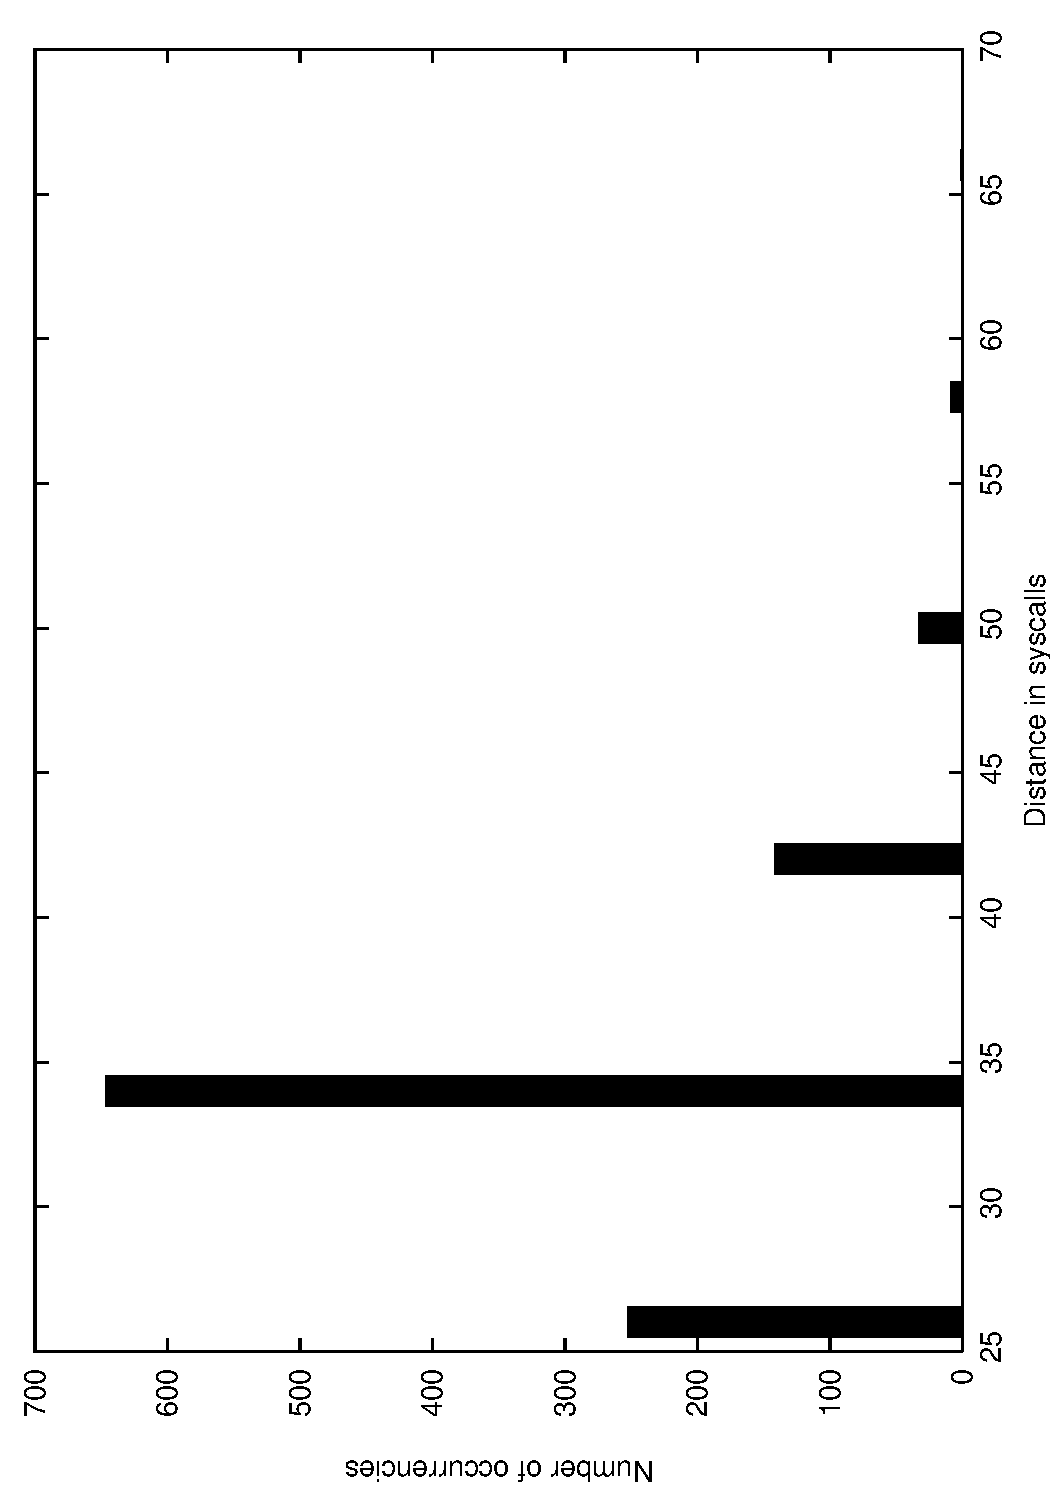
\includegraphics[angle=-90,width=.8\textwidth]{Figures/telnet.pdf}
\caption{\texttt{telnetd}: distribution of the number of other system calls among two \texttt{execve} system calls (i.e., distance between two consecutive \texttt{execve}).}
\label{fig:exectelnet} % etichetta per riferirsi a questa figura col comando \ref{etichettta}
\end{figure}

Riferimento ad una figura è  ``Come si vede in \textsc{Figura~\ref{fig:exectelnet}} \ldots''.


%------------------------------------------------

\section{Bulleted List}

\begin{itemize}
\item $O = $``Intrusion'', $\neg O =$``Non-intrusion'';
\item $A = $``Alert reported'', $\neg A =$``No alert reported''.
\end{itemize}

%------------------------------------------------

\section{Numbered List}

\begin{enumerate}
\item $O = $``Intrusion'', $\neg O =$``Non-intrusion'';
\item $A = $``Alert reported'', $\neg A =$``No alert reported''.
\end{enumerate}

%------------------------------------------------

\section{A Description}

\begin{description}
\item[Time] refers to the use of \emph{timestamp} information, extracted from network packets, to model normal packets. For example, normal packets may be modeled by their minimum and maximum inter-arrival time.
\item[Header] means that the \ac{TCP}\index{TCP} header is decoded and the fields are modeled. For example, normal packets may be modeled by the observed ports range.
\item[Payload] refers to the use of the payload, either at
\ac{IP}\index{IP} or \ac{TCP}\index{TCP} layer. For example, normal packets may be modeled by the most frequent byte in the observed payloads.
\item[Stochastic] means that stochastic techniques are exploited to create models. For example, the model of normal packets may be constructed by estimating the sample mean and variance of certain features (e.g., port number, content length).
\item[Deterministic] means that certain features are modeled following a deterministic approach. For example, normal packets may be only those containing a specified set of values for the \ac{TTL}\index{TTL} field.
\item[Clustering] refers to the use of clustering (and subsequent classification) techniques. For instance, payload byte vectors may be compressed using a \ac{SOM} where class of different packets will stimulate neighbor nodes.
\end{description}

%------------------------------------------------

\section{An Equation}

\begin{equation}
d_a(i,j) := \left\{
\begin{array}{lll}
K_a + \alpha_{a} \delta_{a}(i,j) & \mbox{if the elements are different} \\
0 & \mbox{otherwise}
\end{array}
\right.
\label{eq:distfunction}
\end{equation}

%------------------------------------------------

\section{A Theorem, Proposition \& Proof}

\begin{thm}
$a^2 + b^2 = c^2$
\end{thm}

\begin{prop}
$3 + 3 = 6$
\end{prop}

\begin{proof}
For any finite set $\{p_1,p_2,...,p_n\}$ of primes, consider $m = p_1p_2...p_n+1$. If $m$ is prime it is not in the set since $m > p_i$ for all $i$. If $m$ is not prime it has a prime divisor $p$. If $p$ is one of the $p_i$ then $p$ is a divisor of $p_1p_2...p_n$ and hence is a divisor of $(m - p_1p_2...p_n) = 1$, which is impossible; so $p$ is not in the set. Hence a finite set $\{p_1,p_2,...,p_n\}$ cannot be the collection of all primes.
\end{proof}

%------------------------------------------------

\section{Definition}

\begin{definition}[Anomaly-based \ac{IDS}]
An \emph{anomaly-based \ac{IDS}} is a type of \ac{IDS} that generate alerts $\mathbb{A}$ by relying on normal activity profiles.
\end{definition}

%------------------------------------------------

\section{A Remark}

\begin{rem}
Although the network stack implementation may vary from system to system (e.g., \textsf{Windows} and \textsf{Cisco} platforms have different implementation of \ac{TCP}).
\end{rem}

%------------------------------------------------

\section{An Example}

\begin{example}[Misuse \emph{vs.} Anomaly]\label{ex:misuse-vs-anomaly}
A misuse-based system $M$ and an anomaly-based system $A$ process the same log containing a full dump of the system calls invoked by the kernel of an audited machine. Log entries are in the form:

\begin{center}\small
\begin{verbatim} <function_name>(<arg1_value>, <arg2_value>, ...)
\end{verbatim}
\end{center}
\end{example}

%------------------------------------------------

\section{Note}

\begin{note}[Inspection layer]\label{note:network-stack-standardized}
Although the network stack implementation may vary from system to system (e.g., \textsf{Windows} and \textsf{Cisco} platforms have different implementation of \ac{TCP}), it is important to underline that the notion of IP, TCP, HTTP \emph{packet} is well defined in a system-agnostic way, while the notion of \emph{operating system activity} is rather vague and by no means standardized.
\end{note}
 % qui ci sono esempi di codice per tabelle, figure, etc.

%\section{Introduction}\label{section:Introduction}

Mainstream models of computations focus on one of the two possible directions of computation. 
We typically think how to model 
the way the computation evolves from inputs to outputs while 
we (reasonably) overlook the behavior in the opposite direction, from outputs to inputs. 
Generally speaking, models of computations are neither backward deterministic nor reversible.

For a very rough intuition about what reversible computation deals with, we start by an example.
Let us think about our favorite programming language and think of implementing the
addition between two natural numbers
$ m $ and $ n $. Very likely --- of course without absolute certainty --- we 
shall end up with some procedure \texttt{sum} which takes two arguments and which yields their sum. 
For example, \texttt{sum}($ 3 $,$ 2 $) would yield $ 5 $.
What if we think of asking for the values $ m $ and $ n $ such that \texttt{sum}($ m $,$ n $) = $ 5 $?
If we had implemented \texttt{sum} in a prolog-like language, then we could exploit its 
non deterministic evaluation mechanism to list all the pairs $ (0,5), (1,4), (2,3), (3,2), (4,1) $ and
$ (5,0) $ every of which would well be a correct instance of ($ m, n $). 
In a reversible setting we would obtain
exactly the pair we started from. \Ie, the computation would be backward deterministic.
The interest for the backward determinism arose in the sixties of the last century, 
studying the thermodynamics of computation and the connections between information theory, computability and entropy. 
Since then, the interest for the reversible computing has slowly but incessantly grown.

A forcefully non-exhaustive list of references follows.
Reversible Turing machines are defined in \cite{axelsen11lncs,bennett73ibm,jacopini90siam,lecerf63} while
\cite{axelsen11lncs,axelsen16acta,jacopini89tcs,li1996royal} 
study some of their computational theoretic properties.
Many research efforts have been focused on  boolean functions and cellular 
automata as models of the reversible
computation \cite{Morita2008101,toffoli80lncs}.
Moreover, some research focused on reversible programming languages \cite{DBLP:conf/popl/JamesS12,yokoyama08acm}.
Of course, the interest to build a comprehensive knowledge about reversible computation is wider than 
the mere interest for its computational theoretic aspects. 
The book \cite{perumalla2013chc} is a comprehensive 
introduction to the subject. It spans from low-power-consumption reversible hardware to emerging alternative computational
models like quantum  \cite{guerriniMM15,zorzi14mscs} or bio-inspired \cite{giannini2015tcs} of which reversibility is one the unavoidable building blocks.

\paragraph{Goal} 
The focus of this work is on a \emph{functional model} of reversible computation. 
Specifically, we look for a  sufficiently expressive  class of recursive permutations able to represent all
 Primitive Recursive Functions ($ \PRF $) \cite{rogers1967theory,soare1987book}
whose relevance is sometimes traced to the slogan
``programs which terminate but do not belong to $ \PRF $ are rarely of practical interest.''


We aim at formalizing a language that we identify as Reversible Primitive Permutations ($ \RPP $) and which 
retains the more interesting aspects of $\PRF$.
In analogy to $ \PRF $, our goal is to get a functional characterization of computability
-- but in a reversible setting, of course --- because functions are handier in order to compose 
algorithms. Other models, like, for example, Turing machines-oriented ones are
more convincing from an implementation view-point.
The ability to represent Cantor pairing \cite{rosenberg2009book} is one of the main properties that 
the functional characterization we are looking for must satisfy.
With Cantor pairing available it is possible to express all interesting total properties about the 
traces\footnote{Kleene's $T_n$ predicate, Kleene's normal form theorem and technical tools related to them \cite{cutland1980book,odifreddi1989book,soare1987book}.}
of Turing machines, reversible or not.
The other must-have property of our functional characterization is closure under inversion, which is something
very natural to ask for in a class of permutations and of reversible computing models.

Our quest is challenging because various negative results could have played  against it.
First of all, we remark that the class of all (total) recursive permutations 
cannot be effectively enumerated (see \cite[Exercise 4-6, p.55]{rogers1967theory}). 
In \cite{koz1972ail} a constructive generation of all the recursive permutations is given starting
from primitive recursive permutations. Since no enumeration exists for the latter, none can exist for the former.
Worst, the class of primitive recursive permutations is not closed under inversion \cite{kuznecov50sssr,PaoliniPiccoloRoversiICTCS2015,soare1987book}.
Since the above negative results hold also for the class of elementary permutations 
\cite{cannonito1969jsl,kalimullin03permutations,koz1974ail}, there is no
hope to find any effective description neither of the class of recursive 
permutations nor of the classes of primitive recursive permutations and of elementary permutations.


\paragraph{Comparison with the known literature}
Our quest to identify the reversible  analogous of $ \PRF $  must be throughly related to the following works.
\begin{itemize}
\item 
The programming language $ \mathsf{SRL} $  restricts $ \mathsf{LOOP} $, a language 
for programming $\PRF$ functions \cite{meyer1967acm}. 
Matos introduces $ \mathsf{SRL} $ and some of its variants in \cite{matos03tcs}.
He is the first using $ \Int $ --- the natural numbers with sign --- as the ground type for 
classes of reversible functions.
We share the choice with him.
The work \cite{matos03tcs} focuses on the algebraic aspects of his languages and its relations with 
matrix groups. 

%\todo{Questions 1 and 2, Reviewer 1}
The study of the classes of functions that $ \mathsf{SRL} $ variants can identify
  is part of Matos' work.
Variants of $\mathsf{SRL}$ are complete with respect to reversible boolean circuits \cite{matos2016notes}.
Proving that some given variant of $\mathsf{SRL}$ is $ \mathsf{PRF} $-complete,
i.e. that it represents all the functions in $ \mathsf{PRF} $, naturally ends up with the quest 
to encode the ``test for 0'' like in the proof that $ \mathsf{LOOP} $ and $ \mathsf{PRF} $ are equivalent \cite{meyer1967acm}. 
We \emph{conjecture} that no variant of Matos' languages exists able to simulate a conditional 
control on the flow of execution that, instead, $ \RPP $ contains by definition.
Of course, proving the conjecture false, would promote $\mathsf{SRL}$ to be (in a reasonable sense) the minimal reversible and 
$ \mathsf{PRF} $-complete language.

\item The precursor of this work is \cite{PaoliniPiccoloRoversiICTCS2015}. It introduces the class of functions $ \RPRF $ which is closed by inversion and is $\PRF$-complete. 
The completeness of $ \RPRF $ relies on \emph{built-in} Cantor pairings.
In this paper we show that we can get rid of \emph{built-in} Cantor pairings inside $ \RPP $.
With no \emph{built-in} pairing operators at hand the design of $ \RPP $ relies on operators which are more fine-grained as compared
to the ones used for the definition of $ \RPRF $.
This orients the programming style to enjoy a couple of interesting features.
Inside $ \RPP $ it is natural avoiding to save the entire history of a calculation within a single argument, i.e. into a single ancilla.
This allows to clean the garbage at the end of the simulation of any $ f\in\PRF $, something which is reminiscent of the simulation 
of Turing machines devised in \cite{bennett1989siamjc}.

\item 
Finally we discuss \cite{jacopini89tcs}. 
It introduces the class of reversible functions $ \JMF $ which is as expressive as Kleene's
partial recursive functions \cite{cutland1980book,odifreddi1989book}. 
Therefore, the focus of \cite{jacopini89tcs} is on partial reversible functions while ours  is on total ones. 
The expressiveness of $ \JMF $ is clearly stronger than the one of  $ \RPP $. 
However, we see $ \JMF $ as less abstract than $ \RPP $ for two reasons.
On one side, the primitive functions of $ \JMF $ relies on a given specific binary representation of natural numbers.
On the other, it is not evident that $ \JMF $ is the extension of a total sub-class
analogous to $ \RPP $ which should ideally correspond to $ \PRF $, but in a reversible setting.
\end{itemize}

%%%%%%%%%%%%%%%%%%%%%%%%%%%%
\paragraph{Contents}
We propose a formalism that identifies a class of functions which we call Reversible Primitive Permutations
($ \RPP $) and which is strictly included in the set of permutations.
Section~\ref{section:The class RPP of Reversible Primitive Permutations} defines $ \RPP $ in analogy
with the definition of $ \PRF $, \ie $ \RPP $ is the closure of composition schemes on basic functions.

The functions of $ \RPP $ have identical arity and co-arity and take 
$ \Int $ --- and not only $ \Nat $ --- as their 
domain because $ \Nat $ is not a group. So, $ \RPP $ is sufficiently abstract 
to avoid any reference to any specific 
encoding of numbers and strongly connects our work to Matos' one \cite{matos03tcs}.

For example, in $ \RPP $ we can define a \texttt{sum} that given the two integers $ m $ and $ n $
yields $ m+n $ and $ n $. Let us represent \texttt{sum} as:
\begin{align}
\label{align:sum example}
\arraycolsep=1.4pt
\begin{array}{rcl}
 \left. {\scriptsize \begin{array}{r} m    \\ n \end{array}} \right[
 & \texttt{sum} &
 \left] {\scriptsize \begin{array}{l} m + n\\ n \end{array} } \right.
\end{array}
\enspace .
\end{align}
The implementation of \texttt{sum} inside $ \RPP $ exploits an iteration scheme that iterates $ n $
times the successor, starting on the initial value $ m $ of the first input.
$ \RPP $ implies the existence of a (meta and) \emph{effective} procedure which produces 
the inverse $ \rprInv{f}\in\RPP $ of every given $ f\in\RPP $. 
\Ie, :
\begin{align}
\label{align:diff example}
\arraycolsep=1.4pt
\begin{array}{rcl}
 \left. {\scriptsize \begin{array}{r} p    \\ n \end{array}} \right[
 & \rprInv{\texttt{sum}} &
 \left] {\scriptsize \begin{array}{l} p - n\\ n \end{array} } \right.
\end{array}
\end{align}
belongs to $ \RPP $ and it ``undoes'' \texttt{sum} by iterating $ n $ times
the predecessor on $ p $. So if $ p = m + n $, then $ p - n = m + n - n = m$.
We remark we could have internalized the operation that yields the inverse of a 
function inside $\RPP$ like in \cite{matos03tcs}. We do not internalize it
to avoid mutually recursive definitions in $ \RPP $.

Concerning the \emph{expressiveness}, $ \RPP $ is closed under inversion and it is both $ \PRF $-complete and $ \PRF $-sound.
Completeness is the really relevant property between the two because this means that 
$ \RPP $ subsumes the class $ \PRF $.
This result is in  Section~\ref{section:Completeness of RPP}. It requires quite a lot 
of preliminary work that one can find in Sections~\ref{section:Generalizations inside RPP}, 
\ref{section:A library of functions in TRRF} and~\ref{section:Cantor pairing} 
and whose goal is to encode a bounded minimalization and Cantor pairing. 
The embedding relies on various key aspects of reversible computing. The principal
ones are:  (i) the use of ancillary variables to clone information
and (ii) the compositional programming under the pattern that Bennett's trick dictates
(cf. Section~\ref{section:Some recursion theoretic side effects of RPP}.)

%%%%%%%%%%%%%%%%%%%%%%%%%%%%
\paragraph{Contributions}
 $\RPP$ is a total class of reversible functions closed under inversion, which is $ \PRF $-complete 
and sound. We think that it can play a key role in the setting of reversible computations analogous to that played by $\PRF$ in classical recursion theory.
In particular, it can be used to devise the analogous of Kleene's normal form theorem and Kleene's predicates in the reversible setting;
it can be also used to formalize a reversible arithmetic as the primitive recursive one (a.k.a. Skolem arithmetic).

%As a last remark, we underline that the speculations leading us to the identification
%of $ \RPP $ could slightly widen our foundational perspective on the ``realm'' 
%of (classic and reversible) recursive computations and on their mathematical formalizations. 
%We present our reflections in Section~\ref{section:Some recursion theoretic side effects of RPP} 
%together with (some) possible future work.




%%%%%%%%%%%%%%%%%%%%%%%%% servono ad emacs
%%% Local Variables:
%%% mode: latex
%%% TeX-master: "main.tex"
%%% ispell-local-dictionary: "american"
%%% End: % Include the introduction chapter
%\chapter{A Chapter of Examples}
\label{chapter1}

\section{A Table}

\begin{table}[h]
\centering
\begin{tabular}{rcc}
\toprule \emph{Feature} & \textsc{Misuse-based} &
\textsc{Anomaly-based}\\
    
\midrule Modeled activity: & Malicious & Normal\\
Detection method: & Matching & Deviation\\
Threats detected: & Known & Any\\
False negatives: & High & Low\\
False positives: & Low & High\\
Maintenance cost: & High & Low\\
Attack desc.: & Accurate & Absent\\
System design: & Easy & Difficult\\
\bottomrule
\end{tabular}
\caption[Duality between misuse- and anomaly-based intrusion detection techniques.]{Duality between misuse- and anomaly-based intrusion detection techniques. Note that, an anomaly-based \ac{IDS} can detect ``Any'' threat, under the assumption that an attack always generates a deviation in the modeled activity.}
\label{tab:misuse-vs-anomaly}
\end{table}

%------------------------------------------------

\section{Code}

\begin{pseudoc}
  /* ... */ cd['<'] = {0.1, 0.11} cd['a'] = {0.01, 0.2} cd['b'] =
  {0.13, 0.23} /* ... */

  b = decode(arg3_value);
  
  if ( !(cd['c'][0] < count('c', b) < cd['c'][1]) ||\
       !(cd['<'][0] < count('<', b) < cd['<'][1]) ||\
       ... || ...)  fire_alert("Anomalous content detected!");
  /* ... */
\end{pseudoc}

%------------------------------------------------

\section{A Sideways Table}

\clearpage
\begin{sidewaystable}
\renewcommand{\arraystretch}{1.5} \centering
\begin{tabular}{rcccccc}
\toprule \textsc{Approach} & \textsc{Time} & \textsc{Header} &
\textsc{Payload} & \textsc{Stochastic} & \textsc{Determ.} & \textsc{Clustering}\\
\midrule \citep{phad} & & $\bullet$ & & & & $\bullet$ \\
\citep{kruegel:sac2002:anomaly} & & $\bullet$ & $\bullet$ & $\bullet$ & & \\
\citep{protocolanom} & & $\bullet$ & & $\bullet$ & $\bullet$ & \\
\citep{ramadas} & & & $\bullet$ & & & $\bullet$ \\
\citep{rules-payl} & $\bullet$ & & $\bullet$ & & $\bullet$ & \\
\citep{zanero-savaresi} & & $\bullet$ & $\bullet$ & & & $\bullet$ \\
\citep{wang:raid2004:payl} & & & $\bullet$ & $\bullet$ & & \\
\citep{zanero-pattern} & & $\bullet$ & $\bullet$ & & & $\bullet$ \\
\citep{DBLP:conf/iwia/BolzoniEHZ06} & & $\bullet$ & $\bullet$ & & & $\bullet$ \\
\citep{wang:raid2006:anagram} & & & $\bullet$ & $\bullet$ & & \\
\bottomrule
\end{tabular}
\caption{Taxonomy of the selected state of the art approaches for network-based anomaly detection.}
\label{tab:network-sota-taxonomy}
\end{sidewaystable}
\clearpage

%------------------------------------------------

\section{A Figure}

\begin{figure}[h]
\centering
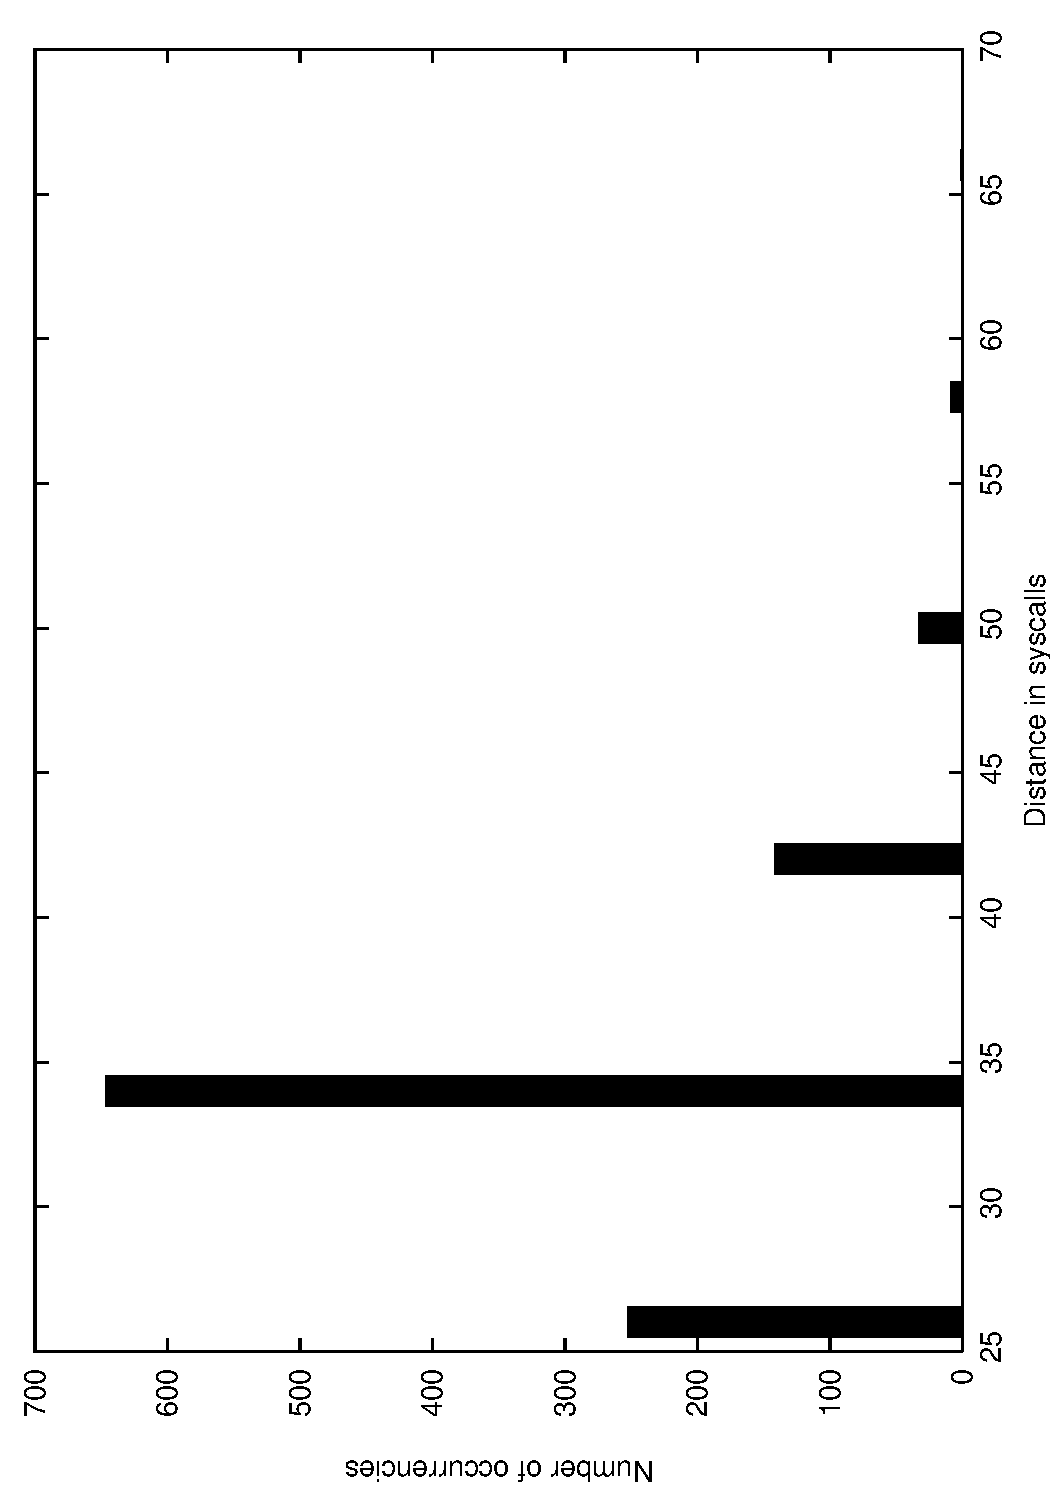
\includegraphics[angle=-90,width=.8\textwidth]{Figures/telnet.pdf}
\caption{\texttt{telnetd}: distribution of the number of other system calls among two \texttt{execve} system calls (i.e., distance between two consecutive \texttt{execve}).}
\label{fig:exectelnet}
\end{figure}

%------------------------------------------------

\section{Bulleted List}

\begin{itemize}
\item $O = $``Intrusion'', $\neg O =$``Non-intrusion'';
\item $A = $``Alert reported'', $\neg A =$``No alert reported''.
\end{itemize}

%------------------------------------------------

\section{Numbered List}

\begin{enumerate}
\item $O = $``Intrusion'', $\neg O =$``Non-intrusion'';
\item $A = $``Alert reported'', $\neg A =$``No alert reported''.
\end{enumerate}

%------------------------------------------------

\section{A Description}

\begin{description}
\item[Time] refers to the use of \emph{timestamp} information, extracted from network packets, to model normal packets. For example, normal packets may be modeled by their minimum and maximum inter-arrival time.
\item[Header] means that the \ac{TCP}\index{TCP} header is decoded and the fields are modeled. For example, normal packets may be modeled by the observed ports range.
\item[Payload] refers to the use of the payload, either at
\ac{IP}\index{IP} or \ac{TCP}\index{TCP} layer. For example, normal packets may be modeled by the most frequent byte in the observed payloads.
\item[Stochastic] means that stochastic techniques are exploited to create models. For example, the model of normal packets may be constructed by estimating the sample mean and variance of certain features (e.g., port number, content length).
\item[Deterministic] means that certain features are modeled following a deterministic approach. For example, normal packets may be only those containing a specified set of values for the \ac{TTL}\index{TTL} field.
\item[Clustering] refers to the use of clustering (and subsequent classification) techniques. For instance, payload byte vectors may be compressed using a \ac{SOM} where class of different packets will stimulate neighbor nodes.
\end{description}

%------------------------------------------------

\section{An Equation}

\begin{equation}
d_a(i,j) := \left\{
\begin{array}{lll}
K_a + \alpha_{a} \delta_{a}(i,j) & \mbox{if the elements are different} \\
0 & \mbox{otherwise}
\end{array}
\right.
\label{eq:distfunction}
\end{equation}

%------------------------------------------------

\section{A Theorem, Proposition \& Proof}

\begin{thm}
$a^2 + b^2 = c^2$
\end{thm}

\begin{prop}
$3 + 3 = 6$
\end{prop}

\begin{proof}
For any finite set $\{p_1,p_2,...,p_n\}$ of primes, consider $m = p_1p_2...p_n+1$. If $m$ is prime it is not in the set since $m > p_i$ for all $i$. If $m$ is not prime it has a prime divisor $p$. If $p$ is one of the $p_i$ then $p$ is a divisor of $p_1p_2...p_n$ and hence is a divisor of $(m - p_1p_2...p_n) = 1$, which is impossible; so $p$ is not in the set. Hence a finite set $\{p_1,p_2,...,p_n\}$ cannot be the collection of all primes.
\end{proof}

%------------------------------------------------

\section{Definition}

\begin{definition}[Anomaly-based \ac{IDS}]
An \emph{anomaly-based \ac{IDS}} is a type of \ac{IDS} that generate alerts $\mathbb{A}$ by relying on normal activity profiles.
\end{definition}

%------------------------------------------------

\section{A Remark}

\begin{rem}
Although the network stack implementation may vary from system to system (e.g., \textsf{Windows} and \textsf{Cisco} platforms have different implementation of \ac{TCP}).
\end{rem}

%------------------------------------------------

\section{An Example}

\begin{example}[Misuse \emph{vs.} Anomaly]\label{ex:misuse-vs-anomaly}
A misuse-based system $M$ and an anomaly-based system $A$ process the same log containing a full dump of the system calls invoked by the kernel of an audited machine. Log entries are in the form:

\begin{center}\small
\begin{verbatim} <function_name>(<arg1_value>, <arg2_value>, ...)
\end{verbatim}
\end{center}
\end{example}

%------------------------------------------------

\section{Note}

\begin{note}[Inspection layer]\label{note:network-stack-standardized}
Although the network stack implementation may vary from system to system (e.g., \textsf{Windows} and \textsf{Cisco} platforms have different implementation of \ac{TCP}), it is important to underline that the notion of IP, TCP, HTTP \emph{packet} is well defined in a system-agnostic way, while the notion of \emph{operating system activity} is rather vague and by no means standardized.
\end{note}
 % Include the first content chapter
%\include{Chapters/chapter2} % Include the second content chapter
%\include{Chapters/chapter3} % Include the third content chapter

\backmatter

\chapterstyle{default} % Reset the chapter style back to the default used for non-content chapters

%----------------------------------------------------------------------------------------
%	BIBLIOGRAPHY
%----------------------------------------------------------------------------------------

\bibliographystyle{plainnat} % Use the plainnat bibliography style

\bibliography{bibliography} % Use the bibliography.bib file as the source of references

%----------------------------------------------------------------------------------------
%	INDEX
%----------------------------------------------------------------------------------------

\printindex % Print the index

%----------------------------------------------------------------------------------------

\end{document}